% =============================================================================
%  BTP progress report: work completed after the midterm presentation.
%
%  Scope: everything from Gaussian process regression onwards. Work presented
%  at the midterm (label construction, transition analysis, hidden Markov model
%  and its leave-one-patient-out validation, growth model) is summarised only
%  as background.
%
%  Every number is taken from saved result files; the values quoted are
%  printed, with their source files, by report/figures/make_post_midterm_sources.py
%  (output: report/BTP_Post_Midterm_Report_sources.txt).
%
%  Figures: ../outputs/step3_gpr/figures/model_comparison.png (existing) and
%  figures/period_slopes.png (plotted from saved bootstrap results by
%  figures/make_period_slopes_figure.py).
% =============================================================================
\documentclass[11pt,a4paper]{article}

\usepackage[T1]{fontenc}
\usepackage[utf8]{inputenc}
\usepackage[margin=2.4cm]{geometry}
\usepackage{graphicx}
\usepackage{amsmath}
\usepackage{amssymb}
\usepackage{booktabs}
\usepackage{tabularx}
\usepackage{float}
\usepackage{caption}
\usepackage{enumitem}
\usepackage[hidelinks]{hyperref}
\usepackage{xurl}

\graphicspath{
  {figures/}
  {../outputs/step3_gpr/figures/}
}

\captionsetup{font=small,labelfont=bf}
\setlist[itemize]{itemsep=2pt,topsep=4pt}
\setlist[enumerate]{itemsep=2pt,topsep=4pt}
\newcolumntype{Y}{>{\raggedright\arraybackslash}X}

\title{\textbf{Motor Subtype Progression in Parkinson's Disease}\\[0.6em]
       \large Progress report: work completed after the midterm presentation}
\author{Parv Patel \quad\textbullet\quad Mayank Tewatia\\[0.4em]
        \small Supervisor: Prof.\ K.~R.\ Sahasranand\\
        \small Department of Data Science, IIT Palakkad}
\date{October 2026}

\begin{document}
\maketitle

\begin{abstract}
\noindent
At the midterm we showed that a patient's recorded motor subtype changes often
and noisily, and that a hidden Markov model predicts the next recorded subtype
of held-out patients with 75.4\% accuracy. This report covers the work done
since then. We forecast the continuous tremor/PIGD ratio with Gaussian process
regression, modelled the tremor and PIGD scores separately, tested whether the
rate of progression changes over follow-up, checked how stable the hidden
Markov model is, and asked whether patients fall into distinct trajectory
groups. The main findings are: flexible models forecast continuous scores
better than simple rules, but this does not translate into better prediction
of the next recorded subtype; PIGD worsens faster than tremor, and the
difference grows gradually over follow-up rather than at a clear transition
point; the three-state hidden Markov model is stable, while larger models add
nothing; and the clustering question remains inconclusive, because we could not
build a sufficiently realistic comparison population without groups.
\end{abstract}

% -----------------------------------------------------------------------------
\section{Introduction and context}

Our project studies how the motor presentation of Parkinson's disease changes
across repeated clinical visits, using the Parkinson's Progression Markers
Initiative (PPMI) cohort \cite{ppmi}. At each visit a patient is classified as
tremor-dominant (TD), postural instability and gait difficulty (PIGD) or
Indeterminate, from the ratio of the mean of 11 tremor items to the mean of 5
gait and balance items of the MDS-UPDRS rating scale \cite{stebbins,goetz}.
A ratio of at least 1.15 is TD, at most 0.90 is PIGD, and values in between
are Indeterminate.

The analysable cohort contains 934 patients with sporadic Parkinson's disease
and at least two labelled visits, with 4,295 labelled visits in total. All
results in this report use this cohort or, where stated, a subset of it.

At the midterm we reported three things that shaped the later work:

\begin{itemize}
  \item The recorded subtype is noisy. About a third (35.2\%) of observed subtype
        changes reverse at the next visit, and a patient's own ratio varies far more
        between visits than the width of the Indeterminate band.
  \item A hidden Markov model (HMM), which treats the true motor state as hidden
        and the recorded label as a noisy reading of it, predicted the next
        recorded subtype of held-out patients with 75.4\% accuracy
        (3,361 predictions), slightly better than simple chains.
  \item A five-state version of the HMM converged in only 404 of 934 folds and
        gave different answers from different starting points.
\end{itemize}

We then proposed four directions: model tremor and PIGD separately rather
than through their ratio; test whether the rate of progression is constant;
ask whether patients fall into distinct progression patterns; and understand
when the HMM fails. This report describes what we did in each direction, and
what we learned.

% -----------------------------------------------------------------------------
\section{Objectives after the midterm}

The work after the midterm was guided by five questions.

\begin{enumerate}
  \item \textbf{Can continuous scores be forecast better than by simple rules?}
        The HMM predicts a category. We wanted to know whether forecasting the
        continuous scores behind the label is more informative.
  \item \textbf{Is the ratio the right quantity to model?} The ratio hides
        severity (2/4 and 10/20 give the same ratio) and is undefined when the
        PIGD score is zero, which happens at 692 of the 4,295 labelled visits.
  \item \textbf{Does the rate of progression change over follow-up?} Every
        earlier model assumed one constant rate.
  \item \textbf{How stable is the HMM, and why does it never predict
        Indeterminate?}
  \item \textbf{Do patient trajectories form distinct, reproducible groups?}
        If so, they could be candidate progression phenotypes.
\end{enumerate}

Running through all five is a sixth question: how much of the variation we see
is caused by measurement noise and by the irregular follow-up of patients,
rather than by the disease itself.

% -----------------------------------------------------------------------------
\section{How the work was evaluated}

All prediction results in this report come from patients the model has not
seen. We use \emph{leave-one-patient-out} validation: each patient is removed
in turn, the model is fitted on the remaining patients, and the removed
patient's visits are predicted one at a time, using only that patient's earlier
visits. This is the same protocol used for the HMM at the midterm.

Every model is compared with simple \emph{baselines}, which are rules that need
no modelling:

\begin{itemize}
  \item \textbf{Persistence}: the next value (or label) equals the last observed
        one. Because labels change slowly on average, this is a strong
        baseline.
  \item \textbf{Patient mean}: the next value equals the patient's own average so
        far.
\end{itemize}

We report the \emph{mean absolute error} (MAE), the average size of a forecast
error, and the \emph{continuous ranked probability score} (CRPS), which judges
the whole predicted distribution, not only its centre; for both, lower is
better \cite{gneiting}. For subtype predictions we report accuracy and
\emph{balanced accuracy}, the average of the accuracies within each of the
three classes, which is fairer when Indeterminate is only about one visit in
ten. Intervals in square brackets are 95\% intervals from resampling patients
(a patient bootstrap); when two models are compared, both are evaluated on the
same resampled patients.

Two cohorts appear below. Models of the ratio can only use visits where the
ratio is defined: 821 patients and 2,707 predicted visits. Models of the
tremor and PIGD scores use all 934 patients and 3,361 predicted visits, which
is exactly the HMM's set. Results from the two cohorts are never compared
directly.

Most of the work was re-run on the college computing cluster. Before any new
experiment, we confirmed that the data panel rebuilt on the cluster is
identical to the one used for the midterm, and that earlier predictions were
reproduced (to within $1.4\times10^{-4}$).

% -----------------------------------------------------------------------------
\section{Work completed}

\subsection{Forecasting the continuous ratio with Gaussian process regression}

\paragraph{Why.} The HMM predicts a category and the midterm growth model
assumed a straight-line trend. We wanted a flexible forecast of the continuous
ratio for each patient, with an honest statement of its uncertainty.

\paragraph{What we did.} Gaussian process regression (GPR) \cite{gpml} predicts
a patient's next value from their earlier visits, using a population trend
plus a smooth, patient-specific deviation from it. How the deviation behaves
over time is set by a \emph{kernel}. We compared a linear-trend kernel (K0,
which reproduces the midterm growth model) with three flexible kernels
(K1--K3), on the 821-patient ratio cohort.

\paragraph{What we found.} The flexible kernels forecast the ratio better than
both the linear-trend model and the baselines (Figure~\ref{fig:gpr}). The MAE
of K1 was 0.972 against 1.043 for persistence, a difference of $-0.071$
[$-0.098$, $-0.045$], and $-0.033$ [$-0.047$, $-0.021$] against K0. The three
flexible kernels were practically identical (K3 minus K1: $-0.0005$
[$-0.0015$, $+0.0005$]). The same ordering held under three alternative ways of
excluding patients with extreme ratios.

However, the better ratio forecasts did not give better subtype predictions.
On the same 2,707 visits, the subtype derived from K1 was correct 72.4\% of the
time, against 73.3\% for persistence, and the GP never predicted Indeterminate.
About 13\% of each predicted distribution lay below zero, a value the ratio
cannot take. Over longer horizons the GP's advantage over persistence looked
larger (MAE 0.976 against 1.605 for forecasts more than five years ahead, 158
forecasts from 100 patients), but these long horizons come only from patients
who stayed in the study for many years, and we did not find a clear widening
within three years.

\begin{figure}[H]
  \centering
  \includegraphics[width=\textwidth]{model_comparison.png}
  \caption{Held-out one-step-ahead forecasts of the TD/PIGD ratio (821 patients,
  2,707 forecasts). Left: mean absolute error; the dashed line marks the best
  simple baseline (persistence). Right: CRPS (lower is better) against the
  share of observations falling inside each model's stated 95\% interval
  (0.95 would be ideal). ``hbayes'' is the midterm growth model and ``K0'' its
  Gaussian process equivalent.}
  \label{fig:gpr}
\end{figure}

\paragraph{What we learned.} Two things. First, flexible forecasting of the
continuous score is possible and beats the simple rules. Second, the ratio is
a poor quantity to forecast: it is undefined for many visits, it cannot be
negative but a Gaussian model allows it to be, and better continuous forecasts
do not help with the subtype label. This led directly to modelling the two
scores separately.

\subsection{Modelling tremor and PIGD scores separately}

\paragraph{Why.} Modelling the tremor and PIGD scores themselves keeps
severity, uses every labelled visit (including the 692 with a PIGD score of
zero), and places the work on exactly the same 3,361 predictions as the HMM, so
the two can finally be compared fairly.

\paragraph{What we did.} We compared, on identical held-out folds and visits:
persistence and patient mean; a joint linear mixed model (LMM, a regression with
a population trend and a patient-specific offset for each score); two separate
Gaussian processes, one per score; and a joint (multi-output) Gaussian process,
which can share information between the two scores. The joint model was fitted
both with and without a cross-score link, so that the link could be tested on
its own. All four kernels (K0--K3) were evaluated held out; earlier, the
slowest two had only been fitted to the whole cohort because of computing time.

\paragraph{What we found.}

\begin{itemize}
  \item \textbf{Trends.} Both scores worsen, PIGD about 2.8 times faster than
        tremor: $+0.066$ per year [$0.059$, $0.073$] against $+0.023$ [$0.017$,
        $0.030$] (linear model, patient bootstrap). The ratio's decline is
        therefore driven by the PIGD score rising, not by tremor improving.
  \item \textbf{Joint modelling gives no benefit.} In 26 of 28 tests of the
        cross-score link the interval included zero. The two exceptions were
        differences of about 0.0005 against a typical error of 0.24. The
        estimated correlation between the two scores was close to zero.
  \item \textbf{Flexible kernels help, but only K2 and K3.} The two kernels with a
        linear trend plus a smooth deviation beat the linear-trend model on
        every probabilistic score for both outcomes (for example PIGD CRPS
        $-0.0035$ [$-0.0053$, $-0.0018$] for K3). K1 did not. An earlier
        conclusion that flexible kernels do not help on the subscores was based
        on K1 alone and is corrected by this result.
  \item \textbf{Against persistence the answer depends on the measure.}
        Persistence still has the smaller average error for PIGD (K3 minus
        persistence: $+0.009$ [$+0.005$, $+0.013$]), but the Gaussian process
        is better when the whole predicted distribution is scored (PIGD CRPS
        $-0.013$ [$-0.015$, $-0.010$]). This second result depends on the
        uncertainty we assigned to persistence.
  \item \textbf{The Gaussian process beats the LMM} on both average error and
        CRPS, for both scores (for example PIGD MAE $-0.022$ [$-0.027$, $-0.017$] for K1).
\end{itemize}

For the next recorded subtype (Table~\ref{tab:subtype}), the Gaussian process
and the HMM were equally accurate (difference $+0.002$ [$-0.005$, $+0.009$]),
and the Gaussian process gave better-calibrated probabilities (lower log loss:
$-0.020$ [$-0.032$, $-0.007$]). The comparison with simply repeating the last
label is more revealing. When each model predicts its most probable class, both
gain about three points of accuracy over repetition, but they do so by never
predicting Indeterminate, and their balanced accuracy is lower. When the
decision rule is adjusted for how common each class is, the HMM is the only
model whose balanced accuracy exceeds simple repetition ($+0.019$ [$+0.007$,
$+0.031$]).

\begin{table}[H]
  \centering
  \small
  \caption{Next recorded subtype, held-out (934 patients, 3,361 predictions).
  ``Most probable'' predicts the class with the highest probability; ``adjusted''
  divides each probability by that class's frequency in the training patients.}
  \label{tab:subtype}
  \begin{tabular}{llccc}
    \toprule
    Model & Decision rule & Accuracy & Balanced accuracy & Indeterminate recall \\
    \midrule
    Repeat last label & -- & 0.723 & 0.548 & 0.193 \\
    HMM & most probable & 0.754 & 0.526 & 0.000 \\
    HMM & adjusted & 0.711 & 0.568 & 0.247 \\
    Gaussian process (K1) & most probable & 0.756 & 0.532 & 0.000 \\
    Gaussian process (K1) & adjusted & 0.650 & 0.554 & 0.220 \\
    \bottomrule
  \end{tabular}
\end{table}

\paragraph{What we learned.} Modelling the scores separately is the better
representation: it uses all visits, shows that PIGD drives the change, and
allows a fair comparison with the HMM. It does not give better prediction of
the next recorded subtype. No model in this work clearly beats repeating the
last label on balanced accuracy except the HMM with an adjusted decision rule.

\subsection{Does the rate of progression change over follow-up?}

\paragraph{Why.} All earlier models assumed a single constant rate. The
midterm listed a changing rate as a hypothesis to test.

\paragraph{What we did.} We fitted the joint mixed model with a rate that is
allowed to change at fixed points (2 and 5 years of follow-up, chosen before
fitting). We then checked this result in several ways: intervals from
resampling patients instead of from the model's own formula; a test for a
change at an unknown time, calibrated by simulating data with a constant rate;
alternative smooth shapes; adjustment for treatment status and disease
duration; and the effect of patients leaving the study.

\paragraph{What we found.} The rate of change is not constant. PIGD worsens
faster later in follow-up, while tremor slows (Figure~\ref{fig:slopes}). The
PIGD rate after five years minus the rate in the first two years was $+0.035$
[$+0.014$, $+0.056$]; for tremor, $-0.020$ [$-0.037$, $-0.002$]. The
calibrated test rejected a constant rate (p $\le 0.005$, the smallest value
possible with 200 simulations).

\begin{figure}[H]
  \centering
  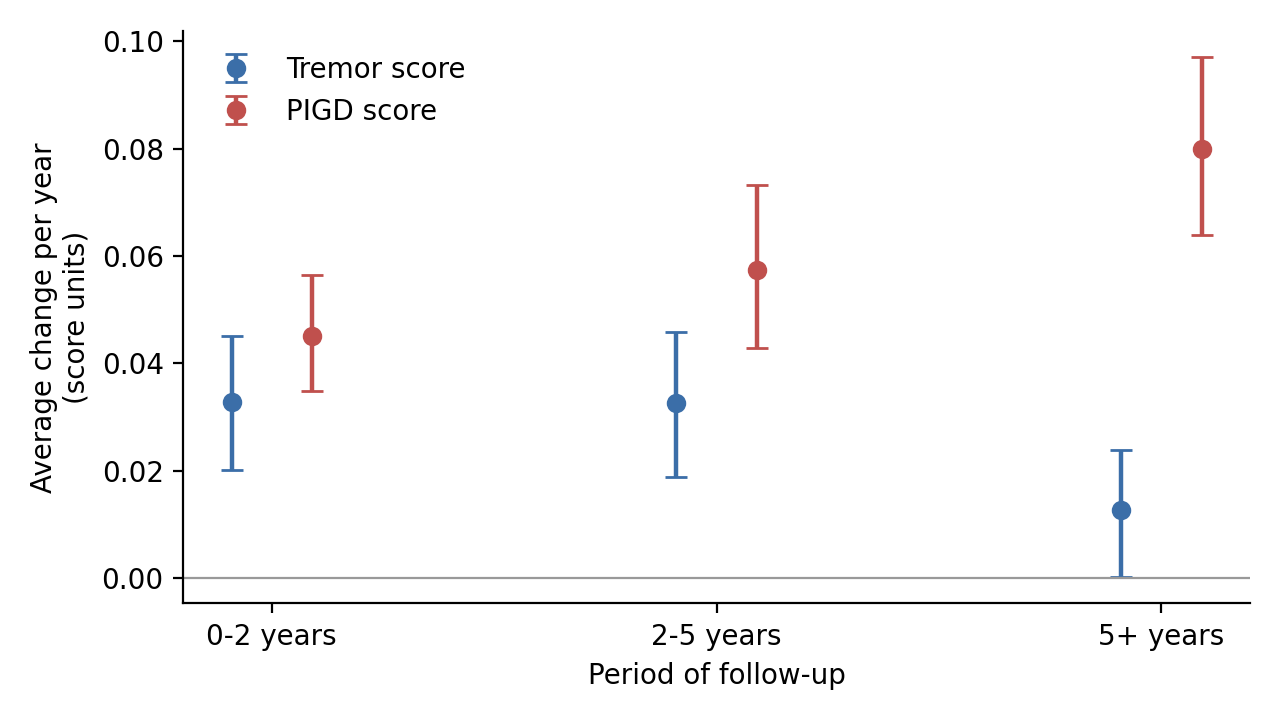
\includegraphics[width=0.72\textwidth]{period_slopes.png}
  \caption{Average yearly change in the tremor and PIGD scores in three periods of
  follow-up, with 95\% intervals from 1,000 patient-bootstrap refits (934
  patients). The rates are population averages from a model with fixed change
  points at 2 and 5 years.}
  \label{fig:slopes}
\end{figure}

Several checks limit how this can be interpreted:

\begin{itemize}
  \item The model's own intervals for the late period were 1.7--2.2 times too
        narrow; the figure shows the corrected ones.
  \item There is no identifiable transition point. The best single change point
        was 4.75 years, but across resampled datasets it ranged from 3 to 9.75
        years (10th to 90th percentile), and a smooth curve fitted the data
        better than any model with change points.
  \item Follow-up time cannot be separated from disease duration. Patients
        joined PPMI within a few years of diagnosis, and after adjusting for
        disease duration the change at five years could no longer be estimated.
  \item Treatment starts in the same period: the share of examinations from
        treated patients rose from 0.10 in the first year to 0.54 in the second
        and about 0.95 after five years.
  \item Patients with higher PIGD scores were more likely to leave the study
        (log-odds $+0.52$ per point [$+0.36$, $+0.71$]). Even so, among the 247
        patients followed for at least six years, PIGD still worsened faster
        late than early ($+0.044$ [$+0.017$, $+0.072$]).
\end{itemize}

Allowing the rate to change improved one-visit-ahead prediction only very
slightly (PIGD CRPS $-0.0010$ [$-0.0017$, $-0.0002$]; no change for tremor).

\paragraph{What we learned.} The divergence between tremor and PIGD is real and
gradual in this cohort. It does not show a biological transition at five years,
and with this study design we cannot say whether it belongs to time in the
study, disease duration or treatment.

\subsection{Stability of the hidden Markov model and the Indeterminate class}

\paragraph{Why.} At the midterm the five-state HMM gave different answers from
different starting points, and no HMM ever predicted Indeterminate. We wanted
to know whether the reported 75.4\% rests on a stable fit, and why
Indeterminate is never chosen.

\paragraph{What we did.} We refitted several HMM versions (three states with
different constraints on how reliably each state is recorded, four states and
five states) from 40 widely spread starting points each. We then evaluated all
of them on held-out patients in ten groups, choosing the version on the training
patients only, so that the reported performance is not biased by the choice.

\paragraph{What we found.}

\begin{itemize}
  \item The three-state HMM used at the midterm reaches the same solution from
        all 40 starting points; its results do not depend on how it is started.
  \item Without its recording-reliability constraint, the three-state model
        reaches the same fit with very different parameters, so its parameters
        cannot be interpreted, although its predictions can be used.
  \item The five-state model stops at its evaluation limit from most starting
        points; with a larger budget it reaches 33 different solutions from 40
        starts. It does not predict better than the three-state model.
  \item When the version is chosen on training patients only, held-out accuracy
        is 0.754 [0.735, 0.774], the same as reported at the midterm.
  \item No version ever gives Indeterminate more than about 0.4
        probability,
        so a most-probable-class rule can never choose it. The probabilities do
        carry some information (they rank true Indeterminate visits above
        others 62\% of the time). With the adjusted decision rule, Indeterminate
        recall rises to 0.25 and balanced accuracy from 0.526 to 0.571, at a
        cost in overall accuracy (0.712).
\end{itemize}

\paragraph{What we learned.} The midterm HMM result is stable and was not
inflated by model choice. Extra hidden states add nothing. The Indeterminate
class is never predicted because of the decision rule combined with weak
information, so overall accuracy alone describes these models poorly; balanced
accuracy and probability scores should be reported with it.

% -----------------------------------------------------------------------------
\section{Summary of important results}

\begin{table}[H]
  \centering
  \small
  \caption{Main results after the midterm. All prediction results are held-out.}
  \label{tab:summary}
  \begin{tabularx}{\textwidth}{>{\raggedright\arraybackslash}p{2.9cm}>{\raggedright\arraybackslash}p{2.9cm}YY}
    \toprule
    Question & Approach & Main finding & What it means \\
    \midrule
    Forecast the continuous ratio better? & Gaussian process regression, 821 patients &
      Beats persistence on MAE ($-0.071$ [$-0.098$, $-0.045$]); subtype accuracy
      0.724 vs 0.733 for persistence & Better continuous forecasts, no better labels;
      the ratio is a poor target \\
    Model tremor and PIGD separately? & LMM, separate and joint Gaussian processes, 934 patients &
      PIGD rises 2.8$\times$ faster than tremor; joint modelling adds nothing;
      K2/K3 beat the linear trend & Better representation, not better subtype prediction \\
    Beat simple repetition on subtype? & GP and HMM vs repeat last label &
      Accuracy equal between GP and HMM; neither beats repetition on balanced
      accuracy except the HMM with an adjusted rule & Next-label prediction is close
      to its limit with these data \\
    Constant rate of progression? & Piecewise mixed model plus checks &
      Rate not constant (p $\le 0.005$); gradual, no identifiable change point &
      Real divergence, but not a demonstrated disease-stage transition \\
    Is the HMM stable? & 40 starts, nested held-out evaluation &
      Three-state model stable; held-out 0.754 [0.735, 0.774]; extra states add nothing &
      The midterm result stands \\
    Distinct trajectory groups? & Reliability audit, simulated comparison populations &
      Inconclusive (Section~\ref{sec:clustering}) & No phenotype claim can be made \\
    \bottomrule
  \end{tabularx}
\end{table}

% -----------------------------------------------------------------------------
\section{The clustering investigation and its conclusion}
\label{sec:clustering}

\paragraph{Motivation.} We wanted to know whether patients form distinct
trajectory groups, such as slow and fast progressors, or whether apparent groups
arise from continuous differences between patients, from measurement noise and
from how often patients were seen.

\paragraph{Are individual trajectories reliable?} We first checked whether each
patient's rate of change can be estimated reliably enough to group patients.
Mostly it cannot. Removing a single visit reversed the direction of the
estimated slope for 369 of 762 patients with three or more visits (tremor) and
for 317 of 762 (PIGD). The median reliability of the patient-specific slope was
0.27 for tremor and 0.53 for PIGD, below the level usually needed to classify
individuals. When each patient's last visit was removed, the agreement between
the new and original two-group clustering (adjusted Rand index, 1 = identical,
0 = chance) was only 0.46.

\paragraph{Why a comparison simulation was needed.} A clustering method always
finds groups, even in data that has none. The fair question is therefore
whether the real data shows stronger or more stable groups than data simulated
from a population with \emph{no} deliberately created groups but with the same
visit schedules, the same score scale and the same measurement noise. If such a
no-groups population produces the same signals, the signals are not evidence
of groups.

\paragraph{First comparison.} Against 200 simulated no-groups populations, the
real data separated into groups much more strongly than expected (a model
selection score, $\Delta$BIC, of 513 against a 95th percentile of 117), but
the groups were no more stable when a visit was removed (agreement 0.750
against a 95th percentile of 0.771). Our pre-specified rule required both, so
clustering was not supported. A later check showed that the simulated
populations were themselves not realistic: the real patients' estimated PIGD
slopes are much more skewed (skewness 2.17, against about 0.4--0.6 in the
simulations), and the simulations produced too many PIGD scores of zero.

\paragraph{Final investigation.} We therefore tried to build a more realistic
no-groups population. Before each attempt we fixed the features it had to
reproduce and the allowed tolerances. If any feature failed, the clustering
comparison was not run. Table~\ref{tab:nulls} summarises the attempts.

\begin{table}[H]
  \centering
  \small
  \caption{Attempts to build a realistic population without groups. Each row was a
  pre-specified check of whether the simulated data reproduces the real data;
  no clustering comparison was run after any failure.}
  \label{tab:nulls}
  \begin{tabularx}{\textwidth}{>{\raggedright\arraybackslash}p{4.4cm}YY}
    \toprule
    Model of the patients and the scores & What it reproduced & What it failed \\
    \midrule
    Skewed, heavy-tailed patient differences on the original score model &
      Most shape targets & PIGD-slope skewness (1.73 vs 2.17); too many zero scores \\
    Three models of the PIGD score (constant noise, noise growing with severity,
      beta-binomial) & Part of the PIGD-slope skew (beta-binomial) &
      Zero scores (about 24\% vs 16\%) and how patients move to zero \\
    Item-level model of the five PIGD items (graded response \cite{samejima}) &
      Zero frequency, item response rates; 14 of 18 targets &
      How often patients stay at or move to zero; PIGD-slope shape \\
    Item-level model plus a slowly varying within-patient deviation &
      14 of 18 targets & The same four targets; the added part was poorly
      determined by the data \\
    \bottomrule
  \end{tabularx}
\end{table}

Two findings came out of this work. First, part of the unusual shape of the
real PIGD slopes comes from the score scale itself: with patient differences
that are not skewed at all, a realistic item-level model already produced a
PIGD-slope skewness of 1.72, against 0.50 for the original simulation. Second,
real patients stay at or leave a PIGD score of zero more persistently than any
model we tried allows. The last model was meant to capture this persistence,
but it fitted a deviation that changes over about 13 years, which over the
available follow-up behaves like a fixed patient offset and was not well
determined by the data.

\paragraph{Conclusion.}

\begin{itemize}
  \item The clustering investigation was closed as inconclusive.
  \item An adequately calibrated no-groups comparison model was not obtained.
  \item The clustering comparison was not run after the pre-specified checks
        failed.
  \item The results do not establish that distinct trajectory groups exist.
  \item The results also do not establish that distinct groups do not exist.
  \item Large differences between patients, or unstable group assignments, are
        not by themselves evidence of distinct clinical phenotypes.
\end{itemize}

% -----------------------------------------------------------------------------
\section{Overall discussion}

\paragraph{Observed directly in the data.} The recorded subtype fluctuates
much more than the underlying disease is likely to. The PIGD score is a sum of
five items that behave very differently: the gait item is scored above zero at
75\% of visits, freezing of gait at 6\%. Scores of zero are common early on,
are not permanent, and become rarer with time. Variation between visits grows
with severity. Follow-up is irregular, and patients with worse gait were more
likely to leave the study.

\paragraph{Supported, but dependent on modelling choices.} PIGD worsens faster
than tremor, and the gap widens over follow-up. Flexible forecasts of the
continuous scores beat simple rules on the measures we used, partly because
of the uncertainty we assigned to the simple rules. The HMM's estimates of
the hidden state are model outputs, not observed clinical truth. Part of the
skew in the patient-specific PIGD slopes is produced by the score scale.

\paragraph{Unresolved.} Whether patients fall into distinct trajectory groups;
why patients near a PIGD score of zero behave more persistently than our models
allow (possible explanations include how individual items are scored near the
floor, changes in item behaviour with treatment or time, or dependence between
successive visits, none of which we have tested); and whether the late
acceleration of PIGD reflects disease stage, treatment or who remained in the
study.

\paragraph{Limitations.} All results come from one cohort (PPMI). The
prediction target is the label produced by our own classification rule, not an
independent clinical diagnosis, so held-out accuracy measures agreement with a
noisy record. Our results concern the next visit; they do not show that an
individual's long-term trajectory can be predicted. Several comparisons with
persistence depend on the uncertainty we assigned to it. Patients who left the
study early are under-represented in the later years.

These limitations are not all failures. Several of them, such as the noisy
label, the effect of the score scale and the confounding of follow-up time with
disease duration, are things we now understand and can state precisely, and
that earlier analyses did not take into account.

% -----------------------------------------------------------------------------
\section{Conclusion}

After the midterm we asked whether continuous forecasting, modelling the two
scores separately, a changing progression rate or trajectory groups could add
to the HMM picture. Continuous forecasting works and beats simple rules on
continuous measures, but it does not predict the next recorded subtype better;
next-label prediction is close to what these data allow, and only the HMM with
an adjusted decision rule improves balanced accuracy over repeating the last
label. Modelling tremor and PIGD separately is the better representation and
shows that PIGD drives the change, with a gradual acceleration that we cannot
attribute to a specific cause. The three-state HMM presented at the midterm is
stable and its accuracy was not inflated. The question of distinct trajectory
groups remains open, because a realistic comparison population could not be
built.

We have not shown that any model can predict an individual patient's long-term
trajectory, and none of the models has been validated for clinical use.

% -----------------------------------------------------------------------------
\section{Future work}

\paragraph{Completed.} All analyses described above are complete, and their
results and settings are recorded in the project repository. The clustering
investigation is closed; we do not plan to restart it.

\paragraph{Proposed.}
\begin{itemize}
  \item Report balanced accuracy and probability scores alongside accuracy in
        every subtype result, and choose any decision rule on training data.
  \item Explore the Indeterminate class further, for example which visits receive
        the highest Indeterminate probability, and whether a sustained
        Indeterminate period means something different from a single visit.
  \item Use the tremor and PIGD scores, and possibly the individual items,
        instead of the ratio wherever the label is not essential.
  \item Study how patients move to and from a PIGD score of zero, as a
        descriptive question about measurement, without building another
        clustering comparison.
  \item Update the earlier explanatory report where its conclusions have been
        corrected, and consolidate everything for the final BTP submission.
\end{itemize}

% -----------------------------------------------------------------------------
\begin{thebibliography}{9}
\bibitem{ppmi} Parkinson Progression Marker Initiative.
  The Parkinson Progression Marker Initiative (PPMI).
  \emph{Progress in Neurobiology}, 95(4):629--635, 2011.
\bibitem{stebbins} G.~T.~Stebbins, C.~G.~Goetz, D.~J.~Burn, J.~Jankovic,
  T.~K.~Khoo, B.~C.~Tilley.
  How to identify tremor dominant and postural instability/gait difficulty
  groups with the Movement Disorder Society Unified Parkinson's Disease Rating
  Scale. \emph{Movement Disorders}, 28(5):668--670, 2013.
\bibitem{goetz} C.~G.~Goetz et~al.
  Movement Disorder Society-sponsored revision of the Unified Parkinson's
  Disease Rating Scale (MDS-UPDRS): scale presentation and clinimetric testing
  results. \emph{Movement Disorders}, 23(15):2129--2170, 2008.
\bibitem{gpml} C.~E.~Rasmussen, C.~K.~I.~Williams.
  \emph{Gaussian Processes for Machine Learning}. MIT Press, 2006.
\bibitem{gneiting} T.~Gneiting, A.~E.~Raftery.
  Strictly proper scoring rules, prediction, and estimation.
  \emph{Journal of the American Statistical Association}, 102(477):359--378, 2007.
\bibitem{samejima} F.~Samejima.
  Estimation of latent ability using a response pattern of graded scores.
  \emph{Psychometrika Monograph Supplement}, No.~17, 1969.
\end{thebibliography}

% -----------------------------------------------------------------------------
\appendix
\section{Models and evaluation, in brief}

\begin{table}[H]
  \centering
  \small
  \begin{tabularx}{\textwidth}{>{\raggedright\arraybackslash}p{3.8cm}Y}
    \toprule
    Term & Meaning in this report \\
    \midrule
    Hidden Markov model (HMM) & The true motor state is hidden and changes over
      time; the recorded label is a noisy reading of it. \\
    Gaussian process regression & Forecasts a patient's next value from their
      earlier visits: population trend plus a smooth patient-specific deviation.
      K0 = linear trend; K1 = smooth deviation; K2, K3 = linear trend plus smooth
      deviation. \\
    Linear mixed model (LMM) & Regression with a population trend and a
      patient-specific offset. \\
    Leave-one-patient-out & Each patient is held out in turn; the model never sees
      the patient it predicts, and only earlier visits are used. \\
    Persistence & Predicts that the next value or label equals the last one. \\
    MAE & Average absolute forecast error. \\
    CRPS & Score of the whole predicted distribution; lower is better. \\
    Balanced accuracy & Average of the accuracies within each class. \\
    $\Delta$BIC & How much better a model with groups fits than one without;
      larger means stronger apparent groups. \\
    Adjusted Rand index & Agreement between two groupings; 1 identical, 0 chance. \\
    \bottomrule
  \end{tabularx}
\end{table}

\section{Sources of the results}

Each number in this report was read from saved result files. A sheet listing
every quoted value next to its source is produced by
\nolinkurl{report/figures/make_post_midterm_sources.py}. The main sources are:
Gaussian process ratio forecasting (\nolinkurl{outputs/step3_gpr/}); the joint
mixed model (\nolinkurl{outputs/joint_subscore/}); the held-out comparison of
subscore models, the HMM stability study and the temporal analysis
(cluster-phase experiment runs, summarised in
\nolinkurl{docs/cluster_phase/04_RESULTS_GENERATED.md}); the clustering audit
(\nolinkurl{outputs/clustering_audit/}) and its closure
(\nolinkurl{docs/cluster_phase/05_FINDINGS.md}, with the specifications and run
records listed there).

\end{document}
